\documentclass[10pt,a4paper,final]{report}
\usepackage[utf8]{inputenc}
\usepackage[english]{babel}
\usepackage{amsmath}
\usepackage{amsfonts}
\usepackage{amssymb}
\usepackage{graphicx}
\author{Gérard Tio Nogueras}
\begin{document}
\chapter{Secure Software}
\section{Development Life cycle}
\textbf{SDLC with Security touchpoints}\\
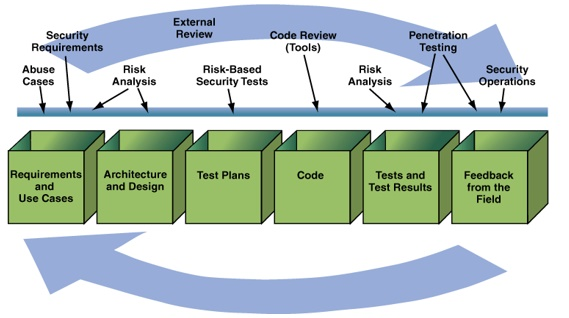
\includegraphics[scale=.65]{cycle.jpg}\\
\textbf{SDL}\\
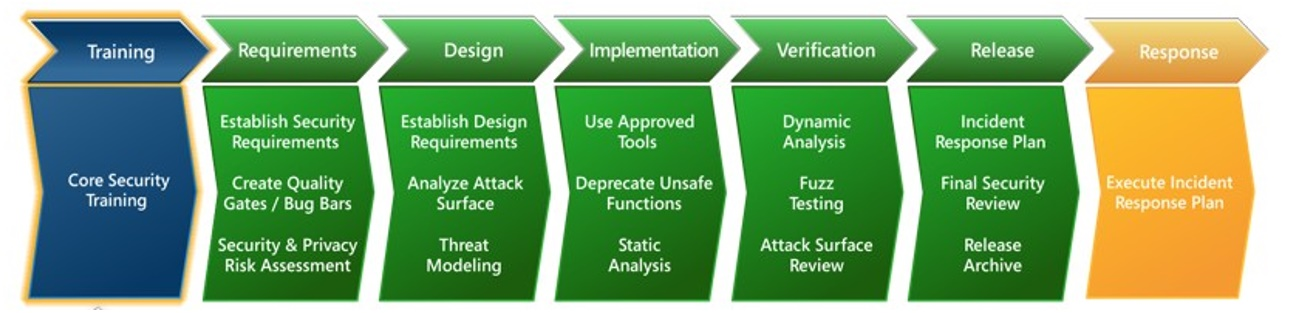
\includegraphics[scale=.35]{SDL.jpg}\\
\subsection{Core Security Training}
General lack of knowledge (barely taught) and progressive learning needed throughout the years.
\subsection{Requirements}
\subsubsection{Security and Privacy Requirements}
Assign experts in security and privacy.
\subsubsection{Create quality bug bar for security and privacy}
Classify the different types of sec and privacy bugs. (moderate, important and critical)\\
Determine priorities for fixes and shipping.\\
Set monitoring of security bugs.
\subsubsection{Security and privacy risk assessment}
Create the security plan, assess timing and resources for the SDL steps.\\
Security risk assessment (critical areas that need review)\\
Privacy risk assessment (give Privacy Impact Ratings(P1,P2,P3) to the different events of the software)
\subsection{Design}
\subsubsection{Establish design requirements}
Design principles: least privilege, compartmentalization,validation of external inputs, logging and auditing of the system, reuse security components and libraries and secure the weakest link.\\
This lead to the specification of a secure architecture, identification of security critical components, secure functional requirements and secure features.
\subsubsection{Attack surface analysis} 
Impossibility of solving all security issues therefore we reduce the attack surface. This means focusing on targets and enablers, channels and protocols and finally access rights.\\
ASA(attack surface analyzer) is a tool to help you identify information on your system attack surface.
\subsubsection{Threat modeling}
Process to find threats, determine their risk and their mitigation.\\
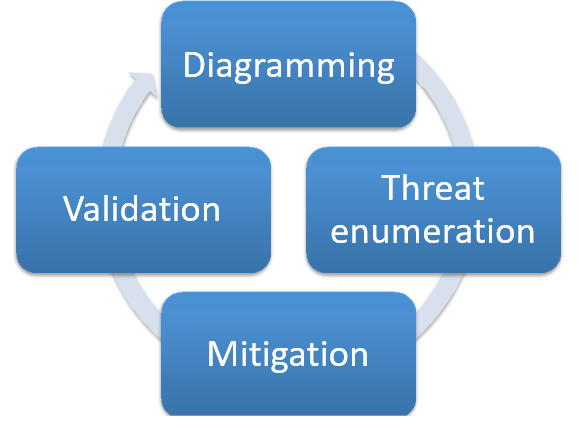
\includegraphics[scale=.65]{ThreatModeling.png}
\subsection{Implementation}
\subsubsection{Use Approved Tools}
Discuss with the employer the approved build tools and options (compilers, static and dynamic analysis, debuggers, Tests verifications, IDE, ...)
\subsubsection{Deprecate Unsafe Functions}
Check for unsafe functions, banned API's and unsafe managed code.
\subsubsection{Perform static analysis}
Identify security vulnerabilities, bug patterns, faster then manual code review, no need of high level of expertise.
\subsection{Verification}
\subsubsection{Perform Dynamic Analysis}
Run-time testing of the functionalities, black box testing and proper functioning of security features(auth, encryption, privacy control, ...).
\subsubsection{Fuzz Testing}
Fuzz testing tools find opportunities for input and will send attack  strings (type of black box testing).
\subsubsection{Attack Surface Review}
ASA to review the attack surface and take corrective action.
\subsection{Release}
\subsubsection{Incident Response Plan, clear definition of support}
Prepare a CSIRP (Cyber Security Incident Response Plan ). This includes contact for Cyber Security, Engineering, marketing and management with decision-making authority. Additionally prepare emergency releases.
\subsubsection{Final Security Review}
Give a view to security ship readiness, provide the FSR(Final security Review = Examination of all SDL activities prior to release, of the threat models, and a review of security tools output + general overview of security performance)
\subsubsection{Release}
Make sure the security plan is completed, the user doc is up to date, archive all the information used for the SDL and final signoffs(authorization)
\subsection{Response}
\subsubsection{Execute Incident Response}
Be ready to execute the Security Response Plan.
\section{Agile}
\subsection{Different Frequency practices}
\subsubsection{One time practices}
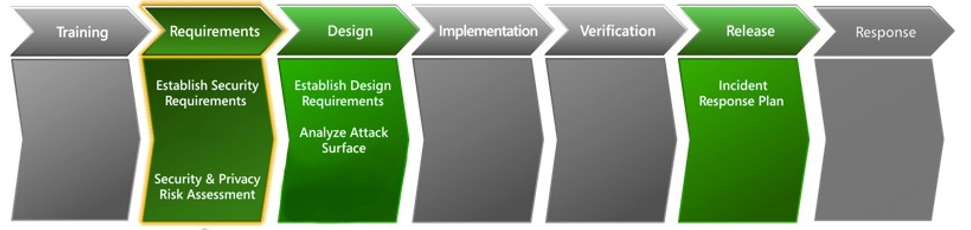
\includegraphics[scale=.53]{oneTime.jpg}\\
Foundational security practices that must be  established once at the start of every new  Agile project.
\subsubsection{Bucket Practices}
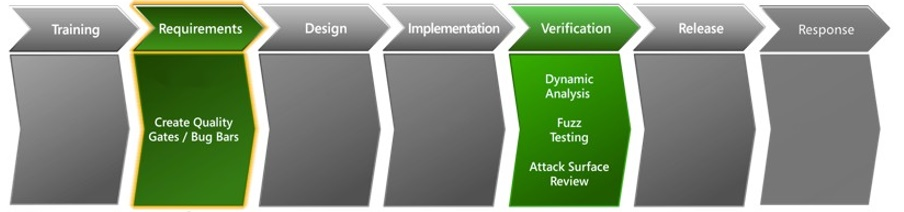
\includegraphics[scale=.55]{bucket.jpg}\\
Important security practices that must be  completed on a regular basis but can be  spread across multiple sprints during the  project lifetime.
\subsubsection{Every-Spring Practices}
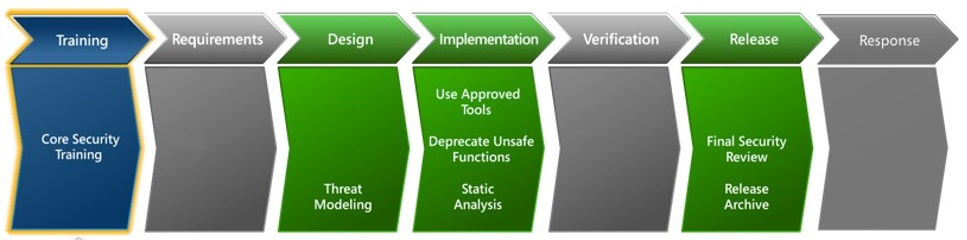
\includegraphics[scale=.53]{sprint.jpg}\\
Essential security practices that should be  performed in every sprint.
\section{Security Usability}
There is this constant problem of balance between usability and security.
Often increased security means less usability. When creating new systems of security that have good usability and no reduced security.
\subsection{Reasons of security failing usability}
User: security is secondary, different backgrounds, little security knowledge, no understanding of the risks and the system.\\
Professionals: Lack of knowledge regarding usability.
\subsection{Importance of usability}
Crimes exploiting human factors are on the rise, humans are the weakest links and humans are easier to hack then systems.
\subsection{Usability Rules}
Easy to learn, efficient to use, easy to remember, likable and less error prone.
\section{Theory of password memory}
\subsection{Problem and Solutions for password learning}
Problem: High difficulty to store long password in human brains.
Solutions: Learning through spaced repetitions
\subsubsection{Steps for Space Repetition for passwords}
\begin{enumerate}
\item Type the password
\item Type the random words displayed
\item Type the random characters as displayed
\item CHECK ONLINE
\end{enumerate}
\section{End-to-End Communications encryptions}
\subsection{Encrypted chat}
More than 1B users, using central key servers and no security UI or fingerprints.\\
Right now you have to trust your provider.\\
For example Facebook is a key, how to verify its state ?
Use multiple social identity providers and ensure that facebook is globally consistent.\\
\section{Password research}
\subsection{Research goal}
Compute the guessing difficulty of given population's distributions and compare them. (cf Foundation)
\section{Security Risk Analysis}
\subsection{Why ?}
Can't secure everything, find the most risky part.
\subsection{What is risk analysis ?}
The whole activity is called \textbf{Risk management}.\\
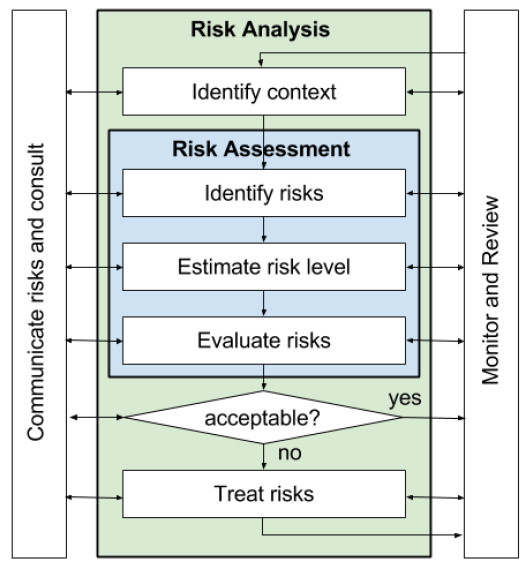
\includegraphics[scale=.55]{RiskManagment.png}\\
\textbf{Risk Analysis} = identifying and ranking risks throughout the SDLC. \\
\textbf{Risk Assessment} = identifying, estimating and evaluating risk.
\subsection{When ?}
Risk analysis comes in when we have on one side \textbf{Assets} and on the other side possible \textbf{vulnerabilities} and \textbf{threats}.\\
The idea is to evaluate the likelihood of the threat event happening and calculate its impact. Combining those values we associate its risk and assess the need of treatment.\\
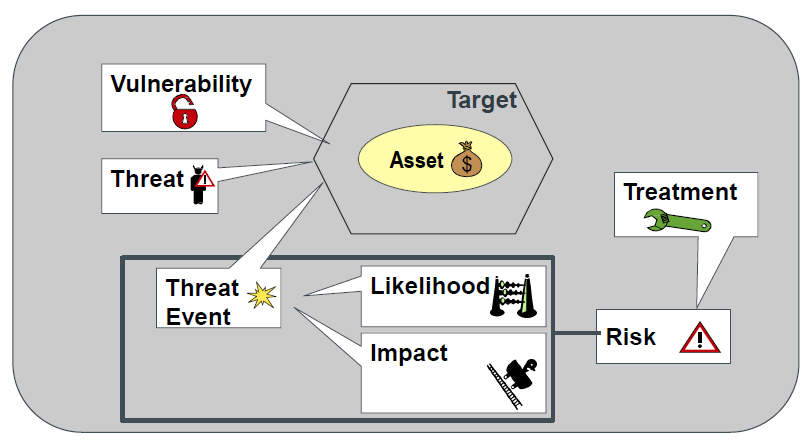
\includegraphics[scale=.55]{RiskModel.png}
\subsection{Risk Process}
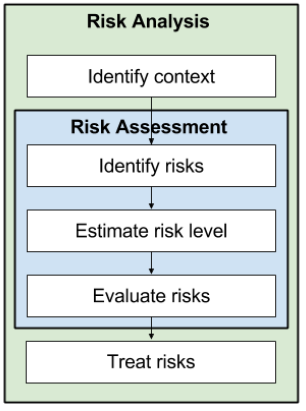
\includegraphics[scale=.75]{RiskProcess.png}
\subsubsection{Identify context}
Identify the target of analysis $=>$ scope of analysis.\\
Identify assets and their value.\\
Specify risk evaluation criteria $=>$ what is tolerated by the client.
\subsubsection{Identify Risks}
Identify threats to assets $=>$ involve owners, users, devs, domain experts and risk analysts.\\
Identify vulnerabilities of assets.
\subsubsection{Evaluate Risks}
Elimination of all risks is impossible.
We need to determine which risks need treatment $=>$ prioritize depending on seriousness.\\
Risk level is a function of the likelihood and impact of a threat event.(quantitative $=>$ a value of loss, qualitative $=>$ high, medium, low.)
\subsubsection{Treat Risks}
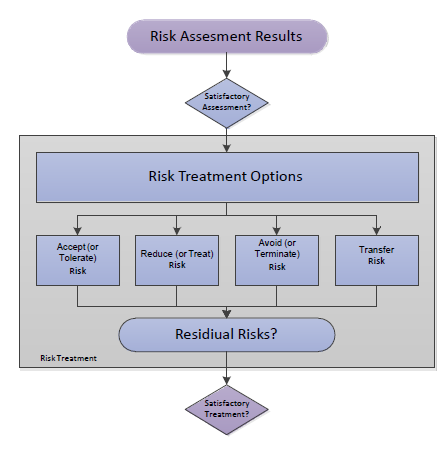
\includegraphics[scale=.75]{RiskTreat.png}
Identify treatments for unaccepted risks.\\
Evaluate and prioritize different treatments with a balance of cost and likelihood.
\section{Risk Analysis Standards}
\subsection{International Standards}
ISO 27001 (process) + ISO\\ 27005(treatments)\\
ISO31000\\
NIST SP800-30 (process) + NIST\\ SP800-53(treatments)
\subsection{National Standards}
IT-Grundschutz(Germany)\\
Magerit(Spain)
\subsection{Standards-based}
OCTAVE\\
CORAS
\section{CORAS}
CORAS is a graphical language that supports the analysis process. It is based on the std ISO31000.
\subsection{CORAS Language}
Different items: \\
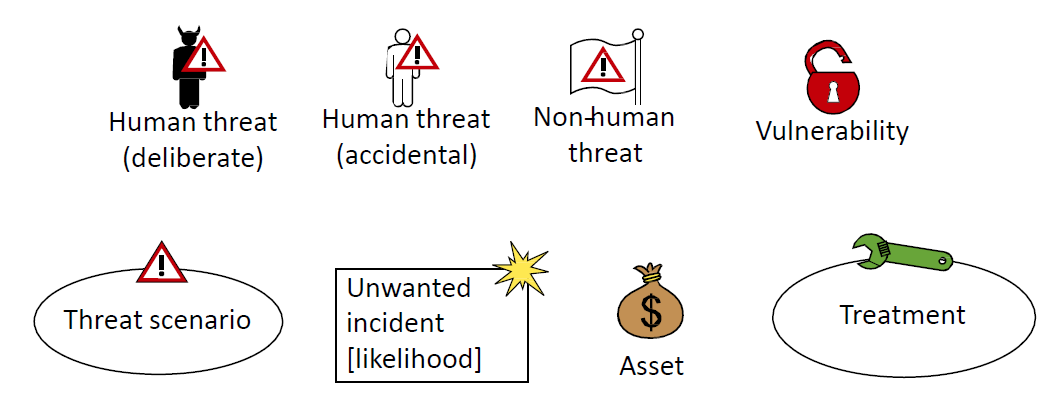
\includegraphics[scale=.4]{CORASItems.png}\\
\subsection{Different types of diagrams}
\subsubsection{Asset Diagram}
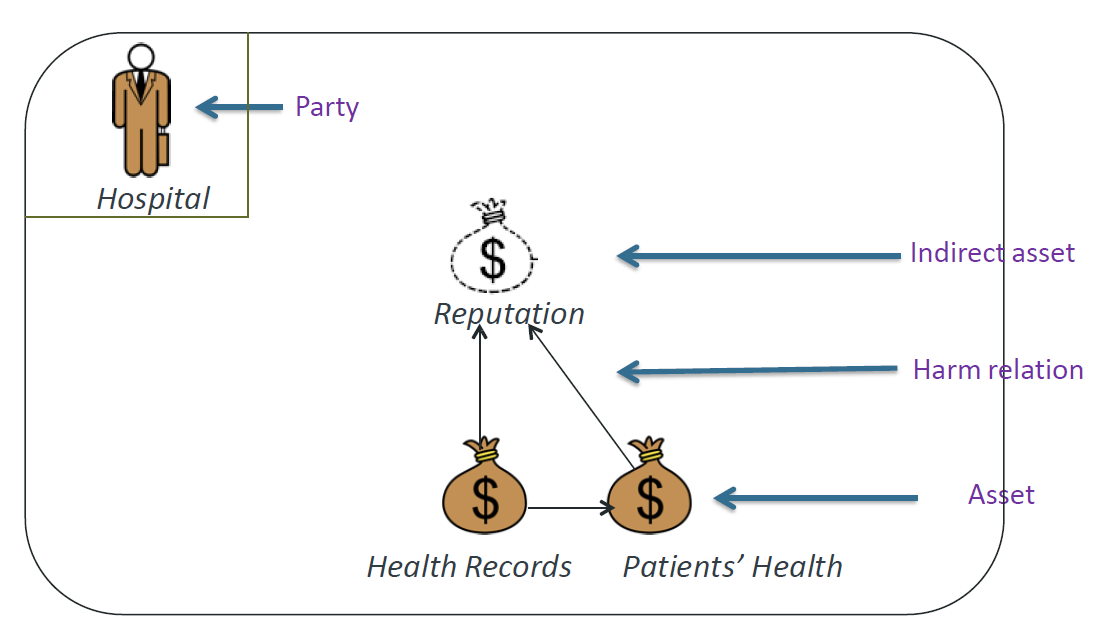
\includegraphics[scale=.4]{AssetDiagram.png}
\subsubsection{Threat Diagram}
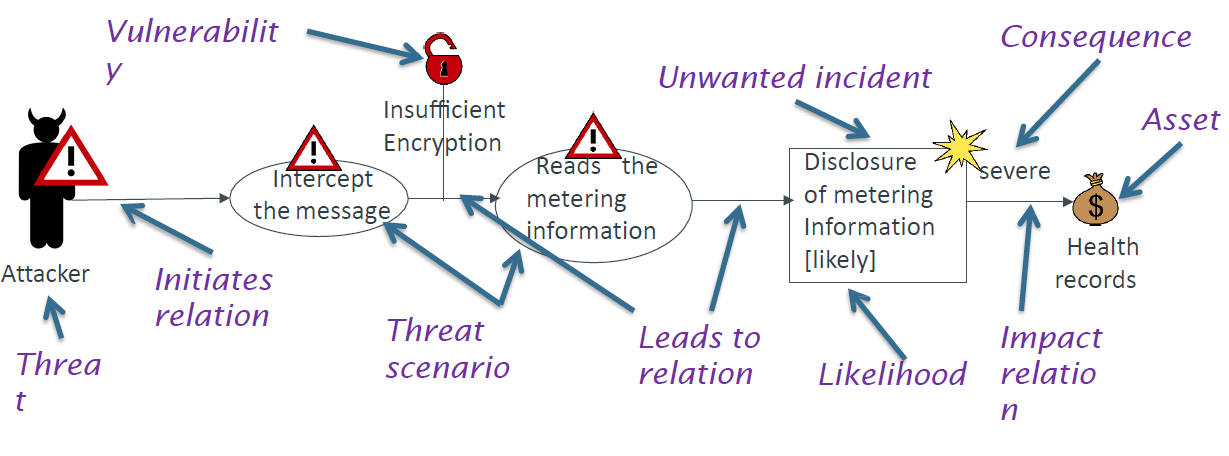
\includegraphics[scale=.4]{ThreatDiagram.png}
\subsubsection{Risk Diagram}
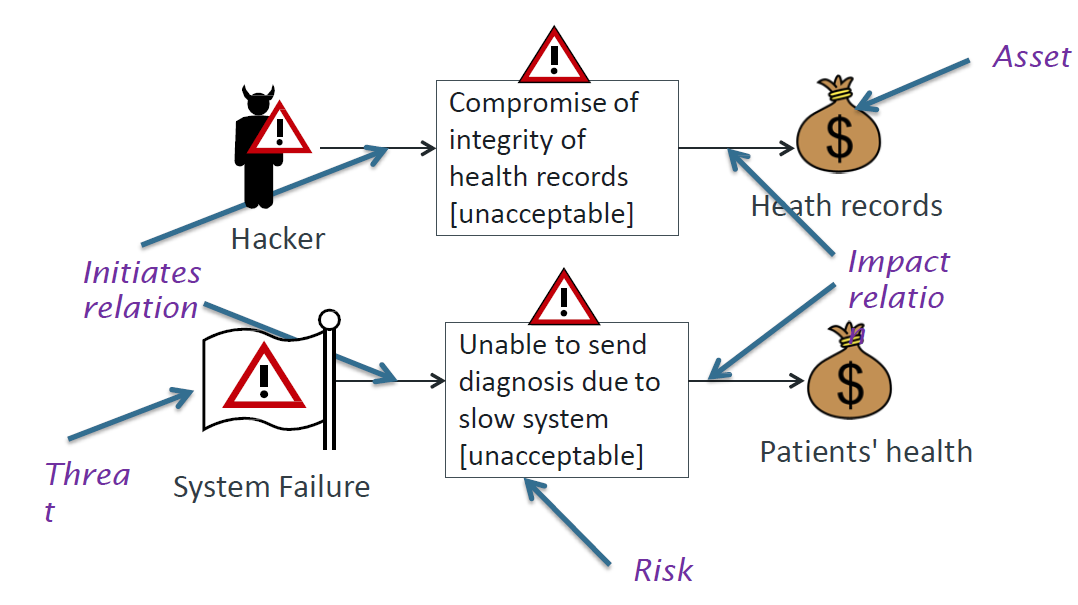
\includegraphics[scale=.4]{RiskDiagram.png}
\subsection{Treatment Diagram}
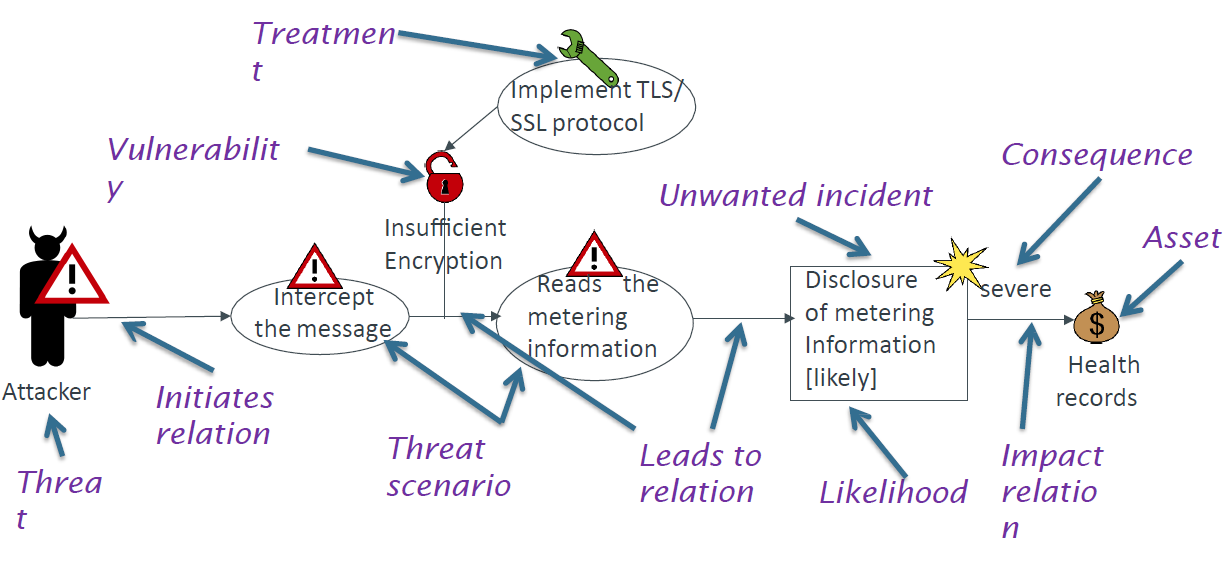
\includegraphics[scale=.4]{TreatmentDiagram.png}
\subsubsection{Treatment Overview Diagram}
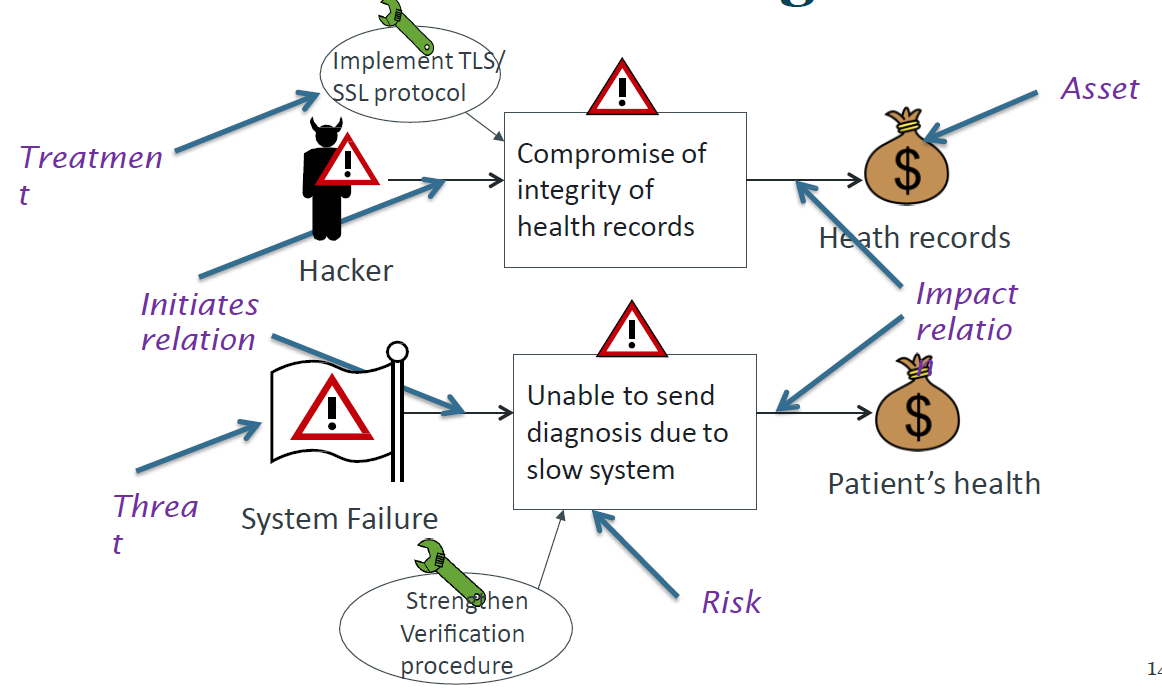
\includegraphics[scale=.4]{OverviewDiagram.png}
\subsection{CORAS Process}
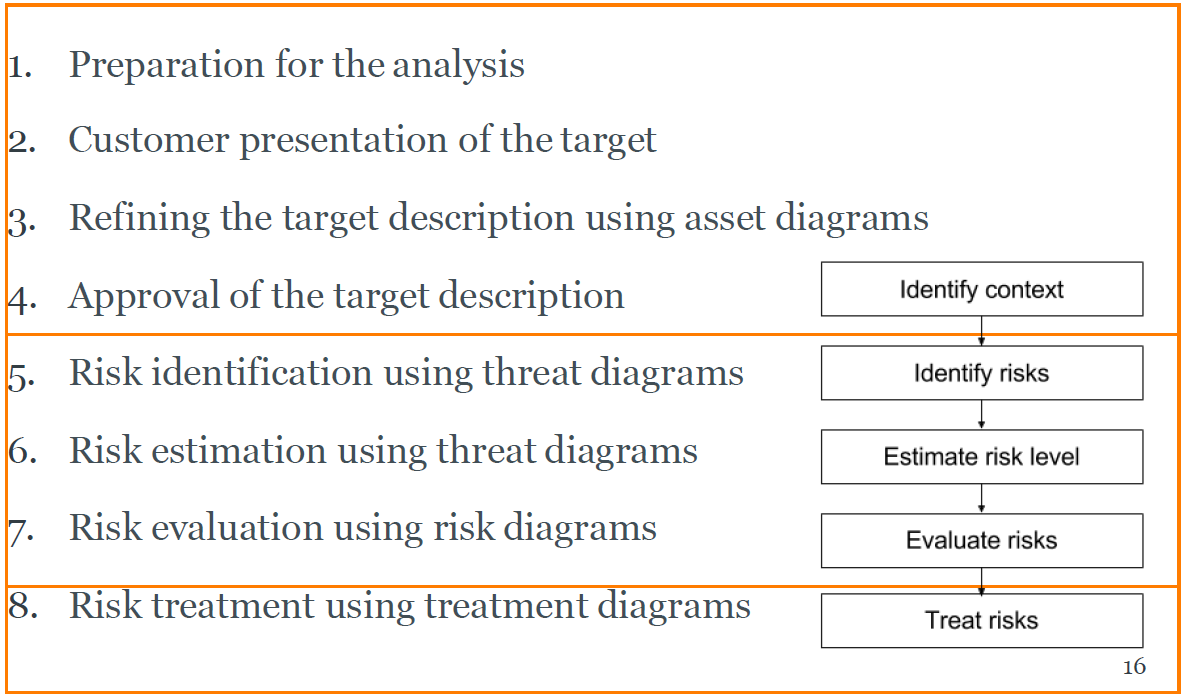
\includegraphics[scale=.4]{CORASProcess.png}
\subsubsection{Let's take an example}
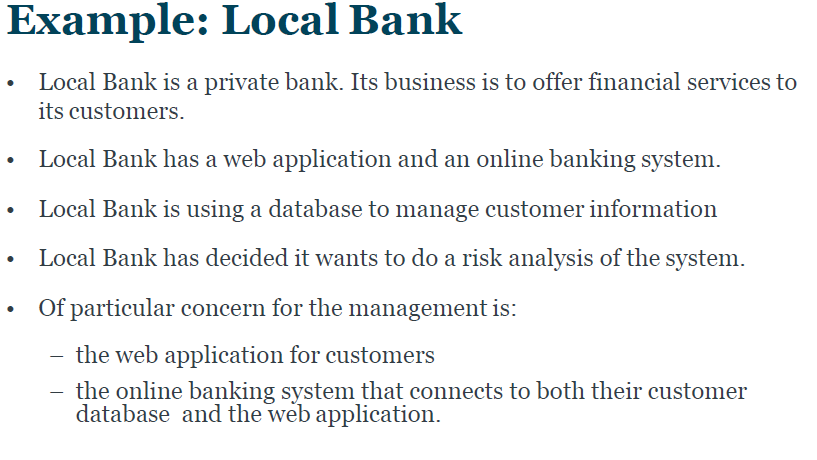
\includegraphics[scale=.55]{Example.png}
\end{document}